\documentclass[11pt]{article}

\usepackage[utf8]{inputenc}
\usepackage{amsmath,amssymb,bm}
\usepackage{booktabs}
\usepackage{caption}
\usepackage{microtype}
\usepackage{times}
\usepackage{algorithm}
\usepackage{algpseudocode}
\usepackage{placeins}
\usepackage{graphicx}
\usepackage{multirow}
\usepackage[a4paper,margin=1in]{geometry}
\usepackage[colorlinks=true,linkcolor=blue,citecolor=blue,urlcolor=blue]{hyperref}
\usepackage[numbers,sort&compress]{natbib}

\renewcommand{\figurename}{Fig.}
\renewcommand{\tablename}{Table}
\renewcommand{\thefigure}{S\arabic{figure}}
\renewcommand{\thetable}{S\arabic{table}}
\renewcommand{\theequation}{S\arabic{equation}}

\title{A Deep Dive into Model Structure: Do Deep Learning Models Learn Verifiable and Transferable Hydrological Knowledge?}
\author{}
\date{}

\begin{document}

\pagenumbering{gobble}

\begin{titlepage}
    \centering
    {\LARGE\bfseries A Deep Dive into Model Structure: Do Deep Learning Models Learn Verifiable and Transferable Hydrological Knowledge?\par}
    \vspace{2.8cm}
    {\Huge\bfseries Supplementary Information\par}
    \vfill
\end{titlepage}

\clearpage
{\hypersetup{linkcolor=black}
    \tableofcontents
}

\clearpage
\pagenumbering{arabic}
\setcounter{page}{1}

\section{Robust Predictive Performance Across Hydrological Stations}
\label{sec:robust_performance}

Interpretability analysis is most meaningful when the underlying predictions are reasonably accurate. We therefore first verify that STEH achieves reliable predictive performance across hydrological stations\cite{ReviewOfXAI}. Predictive skill is evaluated using the NSE, and we follow the commonly used threshold of NSE $>$ 0.5 to indicate satisfactory performance\cite{Nse}.

As shown in Fig.~\ref{nseDistribution}, STEH achieves satisfactory skill for a large proportion of stations, even though it is designed to prioritize interpretability rather than purely optimizing predictive accuracy. Specifically, 327 out of 521 stations (approximately 62.8\%) achieve NSE values greater than 0.5\cite{WRR_RMSE}.

\begin{figure}[ht]
    \centering
    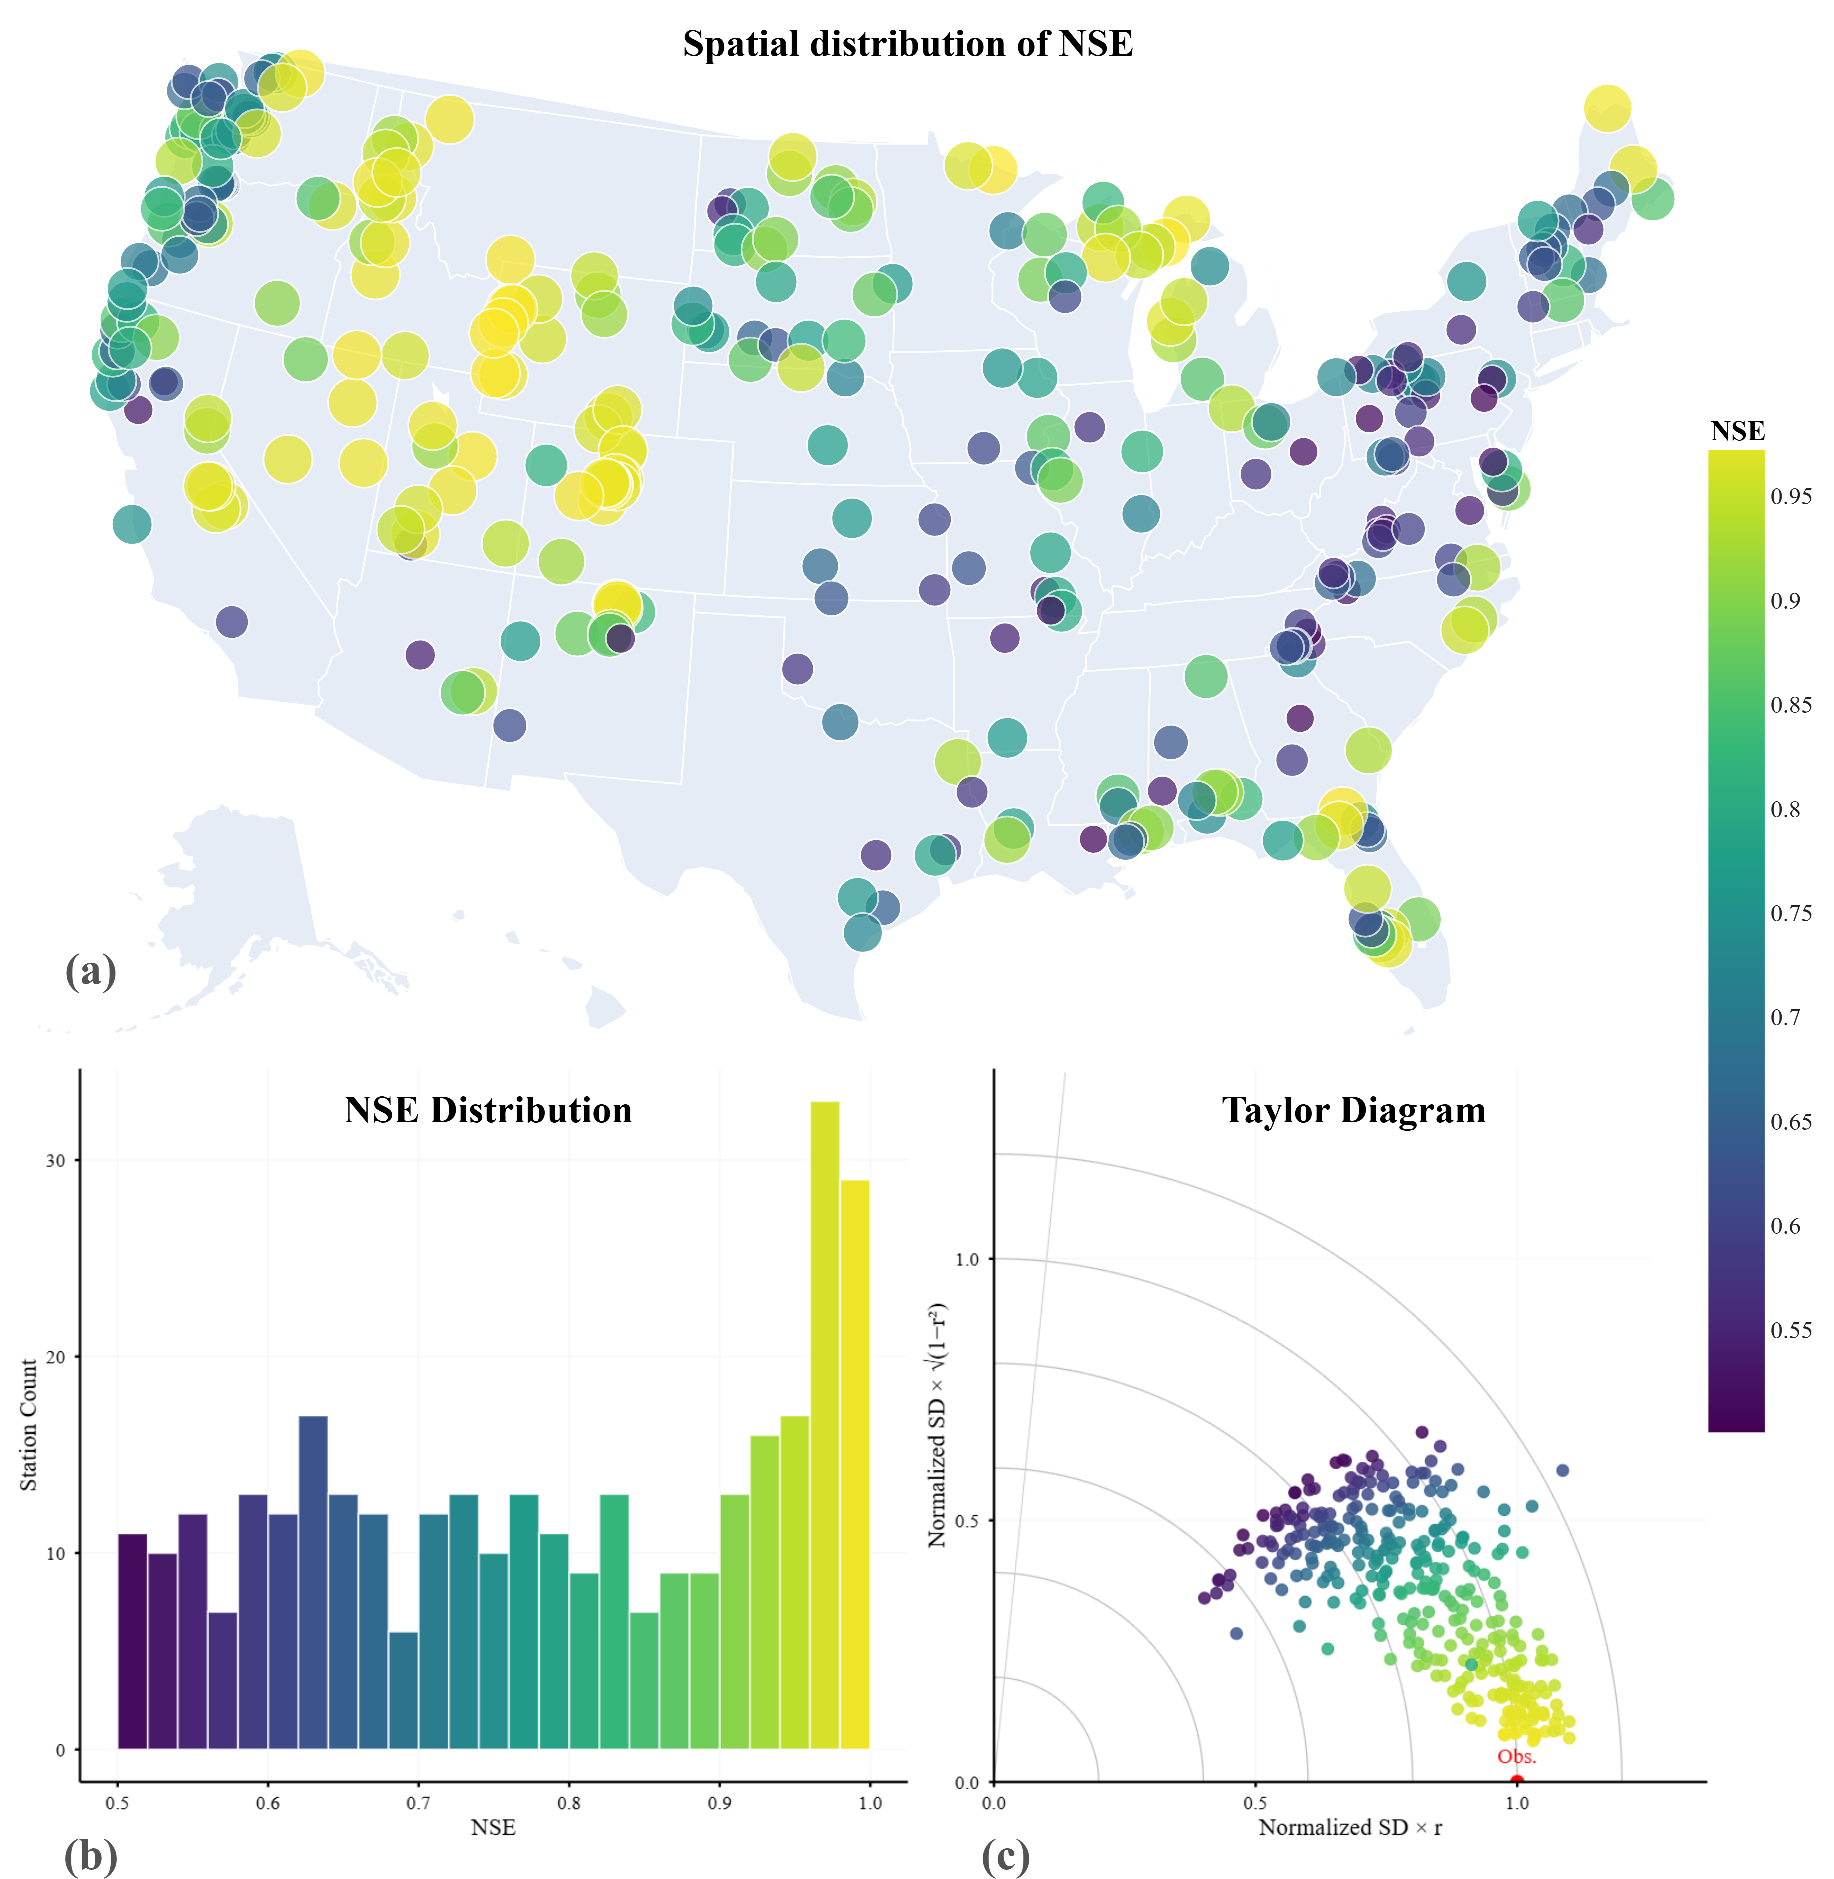
\includegraphics[width=\textwidth]{Figures/Fig3.pdf}
    \caption{\textbf{Model performance across 521 streamflow gauging stations.} (a) Spatial distribution of NSE, with warmer colors indicating higher predictive skill. (b) Distribution of NSE values across all stations, showing that the majority achieve satisfactory performance (NSE $>$ 0.5). (c) Taylor diagram summarizing model performance in terms of correlation, normalized standard deviation, and centered root-mean-square error relative to observations. }
    \label{nseDistribution}
\end{figure}
\FloatBarrier

These results indicate that the model captures key hydrological dynamics in many basins\cite{WRR_NSE}, providing a practical foundation\cite{ReviewOfXAI} for the subsequent interpretability analyses. The insights reported below are therefore grounded in meaningful predictive behavior rather than artifacts of uniformly poor performance\cite{hess-camels}. We next investigate the learned circuit structures and pathways.

\section{Specific Methodological and Data Details}
\label{sec:method}
\subsection{Sparse Transformer}
\subsubsection{Transformer Formulation}

The Transformer architecture has recently been introduced into hydrological time-series modelling because its self-attention mechanism can effectively capture long-range temporal dependencies in hydro-meteorological sequences\cite{LIU2024131389}. In streamflow prediction, antecedent rainfall, temperature, and soil moisture conditions jointly influence discharge responses across multiple time lags, making long-term dependency modelling particularly important\cite{li2024application}.

Let $\mathbf{X}\in\mathbb{R}^{L\times F}$ denote the input sequence with length $L$ and feature dimension $F$. The self-attention operation is defined as\cite{dumontet2026_Transformer_nc}

\begin{equation}
    \mathrm{Attention}(\mathbf{Q},\mathbf{K},\mathbf{V})=
    \mathrm{softmax}\left(\frac{\mathbf{Q}\mathbf{K}^{\top}}{\sqrt{d_k}}\right)\mathbf{V},
\end{equation}
where $\mathbf{Q}$, $\mathbf{K}$, and $\mathbf{V}$ represent the query, key, and value matrices derived from the input representations, and $d_k$ denotes the key dimension used for scaling.

Hidden representations are updated through stacked Transformer encoder blocks\cite{AttentionIsAllYouNeed}:

\begin{equation}
    \mathbf{H}^{(l+1)}=\mathrm{Block}^{(l)}(\mathbf{H}^{(l)}), \quad l=0,\dots,N-1,
\end{equation}
where $\mathbf{H}^{(l)}$ represents the hidden state of layer $l$, and $N$ denotes the number of encoder layers.

\subsubsection{Structured Gating Mechanism}

To enable circuit-level interpretability, structured gating mechanisms are introduced at three levels of the network architecture: input variables, attention heads, and feed-forward neurons\cite{louizos2018learningsparseneuralnetworks}. The effect of gate-based circuit selection is illustrated in Fig.~\ref{fig:sparseTransformer_SI}(e--f).

For the input layer, the gated representation is defined as

\begin{equation}
    \tilde{\mathbf{X}}=\mathbf{X}\odot \mathbf{m}_{\mathrm{in}},
\end{equation}
where $\mathbf{m}_{\mathrm{in}}\in\{0,1\}^{F}$ is a binary mask indicating whether each input feature is retained.

Similarly, head-level and neuron-level masks are defined for each Transformer layer, denoted by $\mathbf{m}_{\mathrm{head}}^{(l)}$ and $\mathbf{m}_{\mathrm{neu}}^{(l)}$, respectively. These masks control the activation of attention heads and feed-forward neurons\cite{TFT}, enabling structured sparsification of the model.

\subsubsection{Sparse Training Strategy}

Training is conducted in three consecutive stages to stabilize optimization and avoid premature pruning of potentially important connections\cite{NIPS2015_three_step_pruning}.

\textbf{Stage I (Origin Model Training).}
The model is first trained without sparsity constraints to establish a stable predictive baseline (Fig.~\ref{fig:sparseTransformer_SI}(a--b)).

\textbf{Stage II (Weight Sparsification).}
Top-$K$ sparsity is progressively imposed on weight tensors with an annealed sparsity schedule\cite{zhu2017prunepruneexploringefficacy} (Fig.~\ref{fig:sparseTransformer_SI}(c--d)):

\begin{equation}
    \rho_t=\rho_{\max}-(\rho_{\max}-\rho_{\min})\left(1-\frac{t}{T}\right)^{\gamma},
\end{equation}
where $\rho_{\min}$ and $\rho_{\max}$ denote the initial and final sparsity ratios. $t$ represents the pruning iteration, $T$ is the total number of steps over which sparsification is applied, and $\gamma$ is a shape parameter that controls the annealing schedule. Specifically, larger $\gamma$ values result in a slower increase in sparsity at early stages and a more rapid transition near the end, while smaller $\gamma$ leads to a more uniform sparsification process.

For each weight group $\mathbf{W}_g$ with $N_g$ elements, the annealed sparsity ratio $\rho_t$ determines the number of retained weights as
\begin{equation}
    k_{g,t}=\max\left(1,\left\lfloor(1-\rho_t)N_g\right\rfloor\right).
\end{equation}
The corresponding magnitude threshold is the $k_{g,t}$-th largest absolute value:
\begin{equation}
    \theta_{g,t}=\operatorname{TopKAbs}(\mathbf{W}_g, k_{g,t})_{\min},
\end{equation}

\textbf{Stage III (Mask Learning).}
Learnable gates are optimized with sparsity regularization (Fig.~\ref{fig:sparseTransformer_SI}(e--f))\cite{NEURIPS2019_1113d7a7}:

\begin{equation}
\left\{
\begin{aligned}
\mathcal{L} &= \mathcal{L}_{\mathrm{task}}+\mathcal{L}_{\mathrm{gate}}, \\
\mathcal{L}_{\mathrm{task}} &= \frac{1}{M}\sum_{n=1}^{M}(\hat{y}_n-y_n)^2, \\
\mathcal{L}_{\mathrm{gate}} &= \lambda_{\mathrm{gate}}\frac{1}{|\mathcal{G}|}\sum_{g\in\mathcal{G}} p_g.
\end{aligned}
\right.
\end{equation}
where $M$ is the number of training samples in a mini-batch, $\mathcal{L}_{\mathrm{task}}$ is the mean squared error loss, $\mathcal{L}_{\mathrm{gate}}$ is the overall gate sparsity regularizer, $\mathcal{G}$ denotes all learnable gates. We consider two types of gates: input-level gates and node-level gates, corresponding to \textit{input} and \textit{head\_neu}, respectively, and $p_g$ is the activation probability of gate $g$.

\begin{figure}[ht]
    \centering
    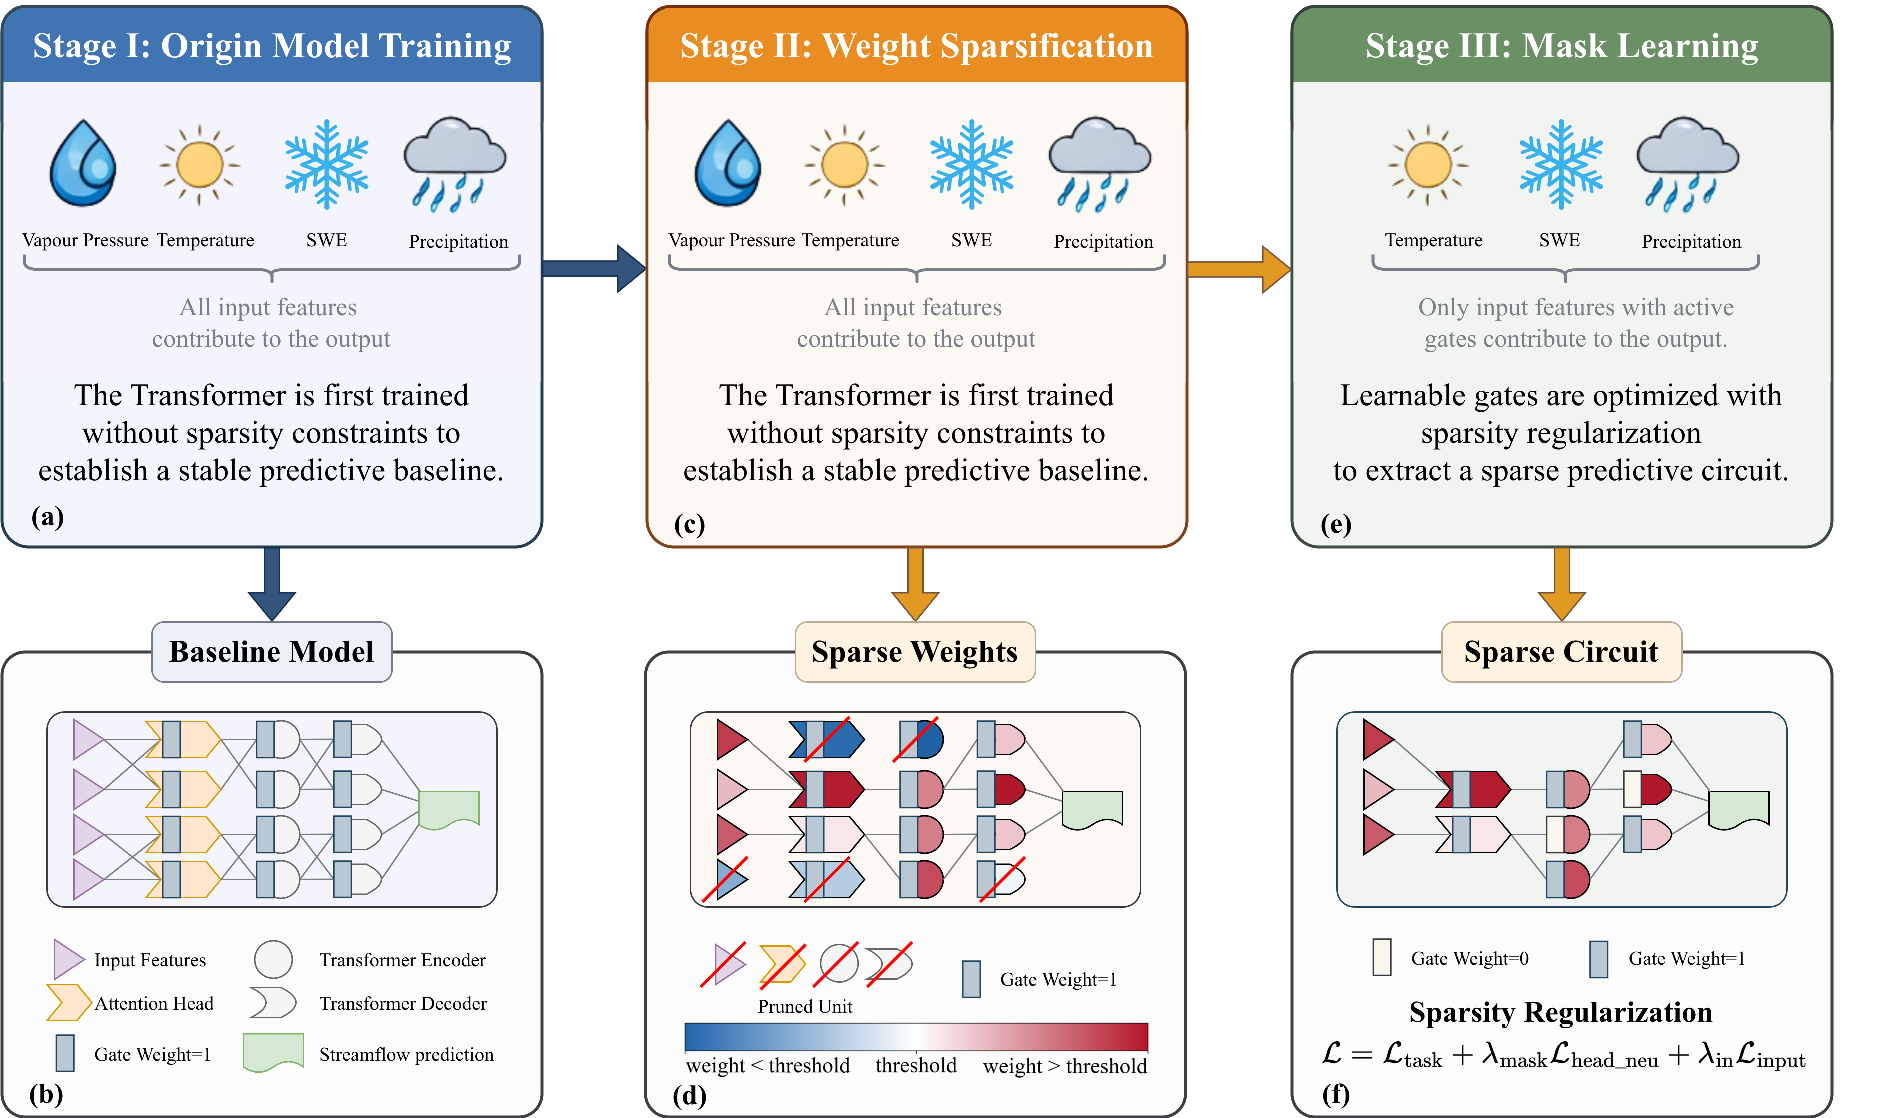
\includegraphics[width=\textwidth]{Figures/Fig2.pdf}
    \caption{\textbf{Three-stage sparsification framework for predictive circuit discovery in Transformer.}
        The model is trained through three stages to progressively transform a dense Transformer into a sparse predictive circuit.
        (a–b) Stage I: Origin model training, where the Transformer is trained without sparsity constraints and all input features contribute to the prediction.
        (c–d) Stage II: Weight sparsification progressively prunes redundant connections according to the sparsity schedule.
        (e–f) Stage III: Mask learning optimizes learnable gates so that only a subset of input features contributes to the final prediction.
        For clarity, only a subset of connections between layers is illustrated in the figure, while the actual model remains fully connected, and decoder attention layers are omitted for simplicity.
        Note that the proposed method does not explicitly modify the network architecture; sparsity is achieved by setting weights or gates to zero, while the visual removal of units in the figure is only for illustrative purposes.
        The number of input variables shown in the figure is fewer than the actual input feature set; this simplification is adopted solely for visual clarity.
    }
    \label{fig:sparseTransformer_SI}
\end{figure}

After training, a compact core predictive circuit is extracted by thresholding gate probabilities\cite{openai_weight_sparse_transformers}. Let $p_i=\sigma(z_i)$ denote the activation probability of gate $i$. A unit is retained if

\begin{equation}
    a_i=\mathrm{I}(p_i>\tau),
\end{equation}
where $\tau$ is the pruning threshold, which is optimized by BO algorithm. Applying this rule to all gates yields a compact model containing only the most important computational pathways.

\subsection{Interpretability Analysis}

\subsection*{(1) Ablation-based Importance}

To quantify the structural importance of individual computational units, targeted ablation is applied to each candidate unit $u$~\cite{morcos2018importancesingledirectionsgeneralization}. The importance score is defined as

\begin{equation}
    \Delta \mathrm{MSE}_{u}=\mathrm{MSE}(\mathrm{ablate}(u))-\mathrm{MSE}(\mathrm{base}).
    \label{eq:Delta_MSE}
\end{equation}

Unlike gradient-based attribution methods, this intervention-based measurement directly evaluates the structural contribution of each component by observing the performance change after structural removal\cite{wang2022interpretabilitywildcircuitindirect}.

\subsection*{(2) Interaction Analysis}

To analyze dependencies between components, pairwise interaction scores are defined as

\begin{equation}
    I_{ij}=\Delta_{ij}-\Delta_i-\Delta_j.
    \label{eq:interaction}
\end{equation}

Positive values indicate synergistic interactions, whereas negative values suggest redundancy or functional substitution.

\subsection*{(3) Top-K Faithfulness}

To evaluate the trade-off between circuit compactness and predictive fidelity, a top-$K$ faithfulness analysis is conducted by retaining only the most important units and measuring the resulting performance degradation\cite{7552539}.

\subsection*{(4) Physical Probing}

To examine whether hidden representations encode physically meaningful hydrological information, linear probes are applied to hidden states\cite{pmlr-v97-verma19a}.

Let $\mathbf{h}_n\in\mathbb{R}^{D}$ denote the hidden representation of sample $n$. The probe model is defined as

\begin{equation}
    \hat{y}_n^{\mathrm{phys}}=\mathbf{w}^{\top}\mathbf{h}_n+b,
\end{equation}
where $\mathbf{w}$ and $b$ are parameters estimated using least squares regression.

Probe performance is evaluated using the coefficient of determination ($R^2$). To avoid probe overfitting, the probe model is intentionally restricted to a simple linear form without hidden layers.

Representative hydrological variables such as cumulative rainfall\cite{PIRONE2023128949}, antecedent precipitation index (API)\cite{CAMELS}, and rainfall change rate are used as probe targets. Let $P_t$ denote precipitation at day $t$, and let $W$ be the look-back window length. Their definitions are

\begin{equation}
    R^{\mathrm{cum}}_t(W)=\sum_{k=0}^{W-1} P_{t-k},
\end{equation}

\begin{equation}
    \mathrm{API}_t(W,\kappa)=\sum_{k=0}^{W-1}\kappa^{k}P_{t-k}, \qquad 0<\kappa<1,
\end{equation}

\begin{equation}
    R^{\mathrm{chg}}_t=\frac{P_t-P_{t-1}}{P_{t-1}+\varepsilon},
\end{equation}
where $\kappa$ is a decay factor controlling the memory of antecedent rainfall and $\varepsilon$ is a small constant to avoid division by zero.

\subsection{Evaluation Metrics}

Model evaluation is conducted from three perspectives: predictive accuracy, explainability properties, and hydro-climatic diagnostics.

Predictive accuracy is measured using standard hydrological metrics including RMSE\cite{WRR_RMSE}, MAE\cite{WRR_MAE}, and NSE\cite{WRR_NSE}. Explainability-related metrics include ablation importance ($\Delta\mathrm{MSE}$, Eq.~\ref{eq:Delta_MSE}), interaction score ($I_{ij}$, Eq.~\ref{eq:interaction}), and top-$K$ faithfulness\cite{7552539} trends. Structural sparsity statistics are also reported to quantify circuit compactness.

Hydro-climatic diagnostics are used to characterize the climatic regimes of catchments. Let $\bar{P}$, $\overline{\mathrm{PET}}$, and $\bar{Q}$ denote the long-term mean annual precipitation, potential evapotranspiration, and streamflow, respectively, and let $P_m$ ($m=1,\dots,12$) be the mean monthly precipitation with $\bar{P}_{\mathrm{ann}}=\sum_{m=1}^{12}P_m$.

The \textbf{aridity index} (AI)\cite{zomer2022version} describes the balance between water supply and atmospheric demand:
\begin{equation}
    \mathrm{AI}=\frac{\bar{P}}{\overline{\mathrm{PET}}}.
\end{equation}
Values $\mathrm{AI}<1$ indicate arid conditions, while $\mathrm{AI}>1$ indicates humid conditions.

The \textbf{Streamflow coefficient} ($C_r$)\cite{WRR_coefficient} represents the fraction of precipitation that becomes streamflow:
\begin{equation}
    C_r=\frac{\bar{Q}}{\bar{P}}.
\end{equation}

The \textbf{precipitation seasonality index} (SI)\cite{SI} quantifies the degree of seasonal concentration of rainfall:
\begin{equation}
    \mathrm{SI}=\frac{1}{\bar{P}_{\mathrm{ann}}}\sum_{m=1}^{12}\left|P_m-\frac{\bar{P}_{\mathrm{ann}}}{12}\right|,
\end{equation}
where $\mathrm{SI}=0$ indicates perfectly uniform monthly distribution and larger values correspond to stronger seasonal concentration. Together, these three diagnostics are used to stratify stations by hydro-climatic regime and to contextualize model performance across different environmental conditions.

\subsection{Data}
\label{sec:data}
Because streamflow record availability varies across stations, we apply a unified quality-control procedure within this period. Stations with more than 100 missing daily values in the target streamflow series are excluded, whereas stations with at most 100 missing days are retained and missing values are filled by linear interpolation. After preprocessing, 521 stations remain for subsequent analysis, as Fig~\ref{fig:station} shows. All retained stations provide multi-year continuous records over the common window (well beyond 20 years), ensuring sufficient sample size for deep learning training.

\begin{figure*}[htbp]
    \centering
    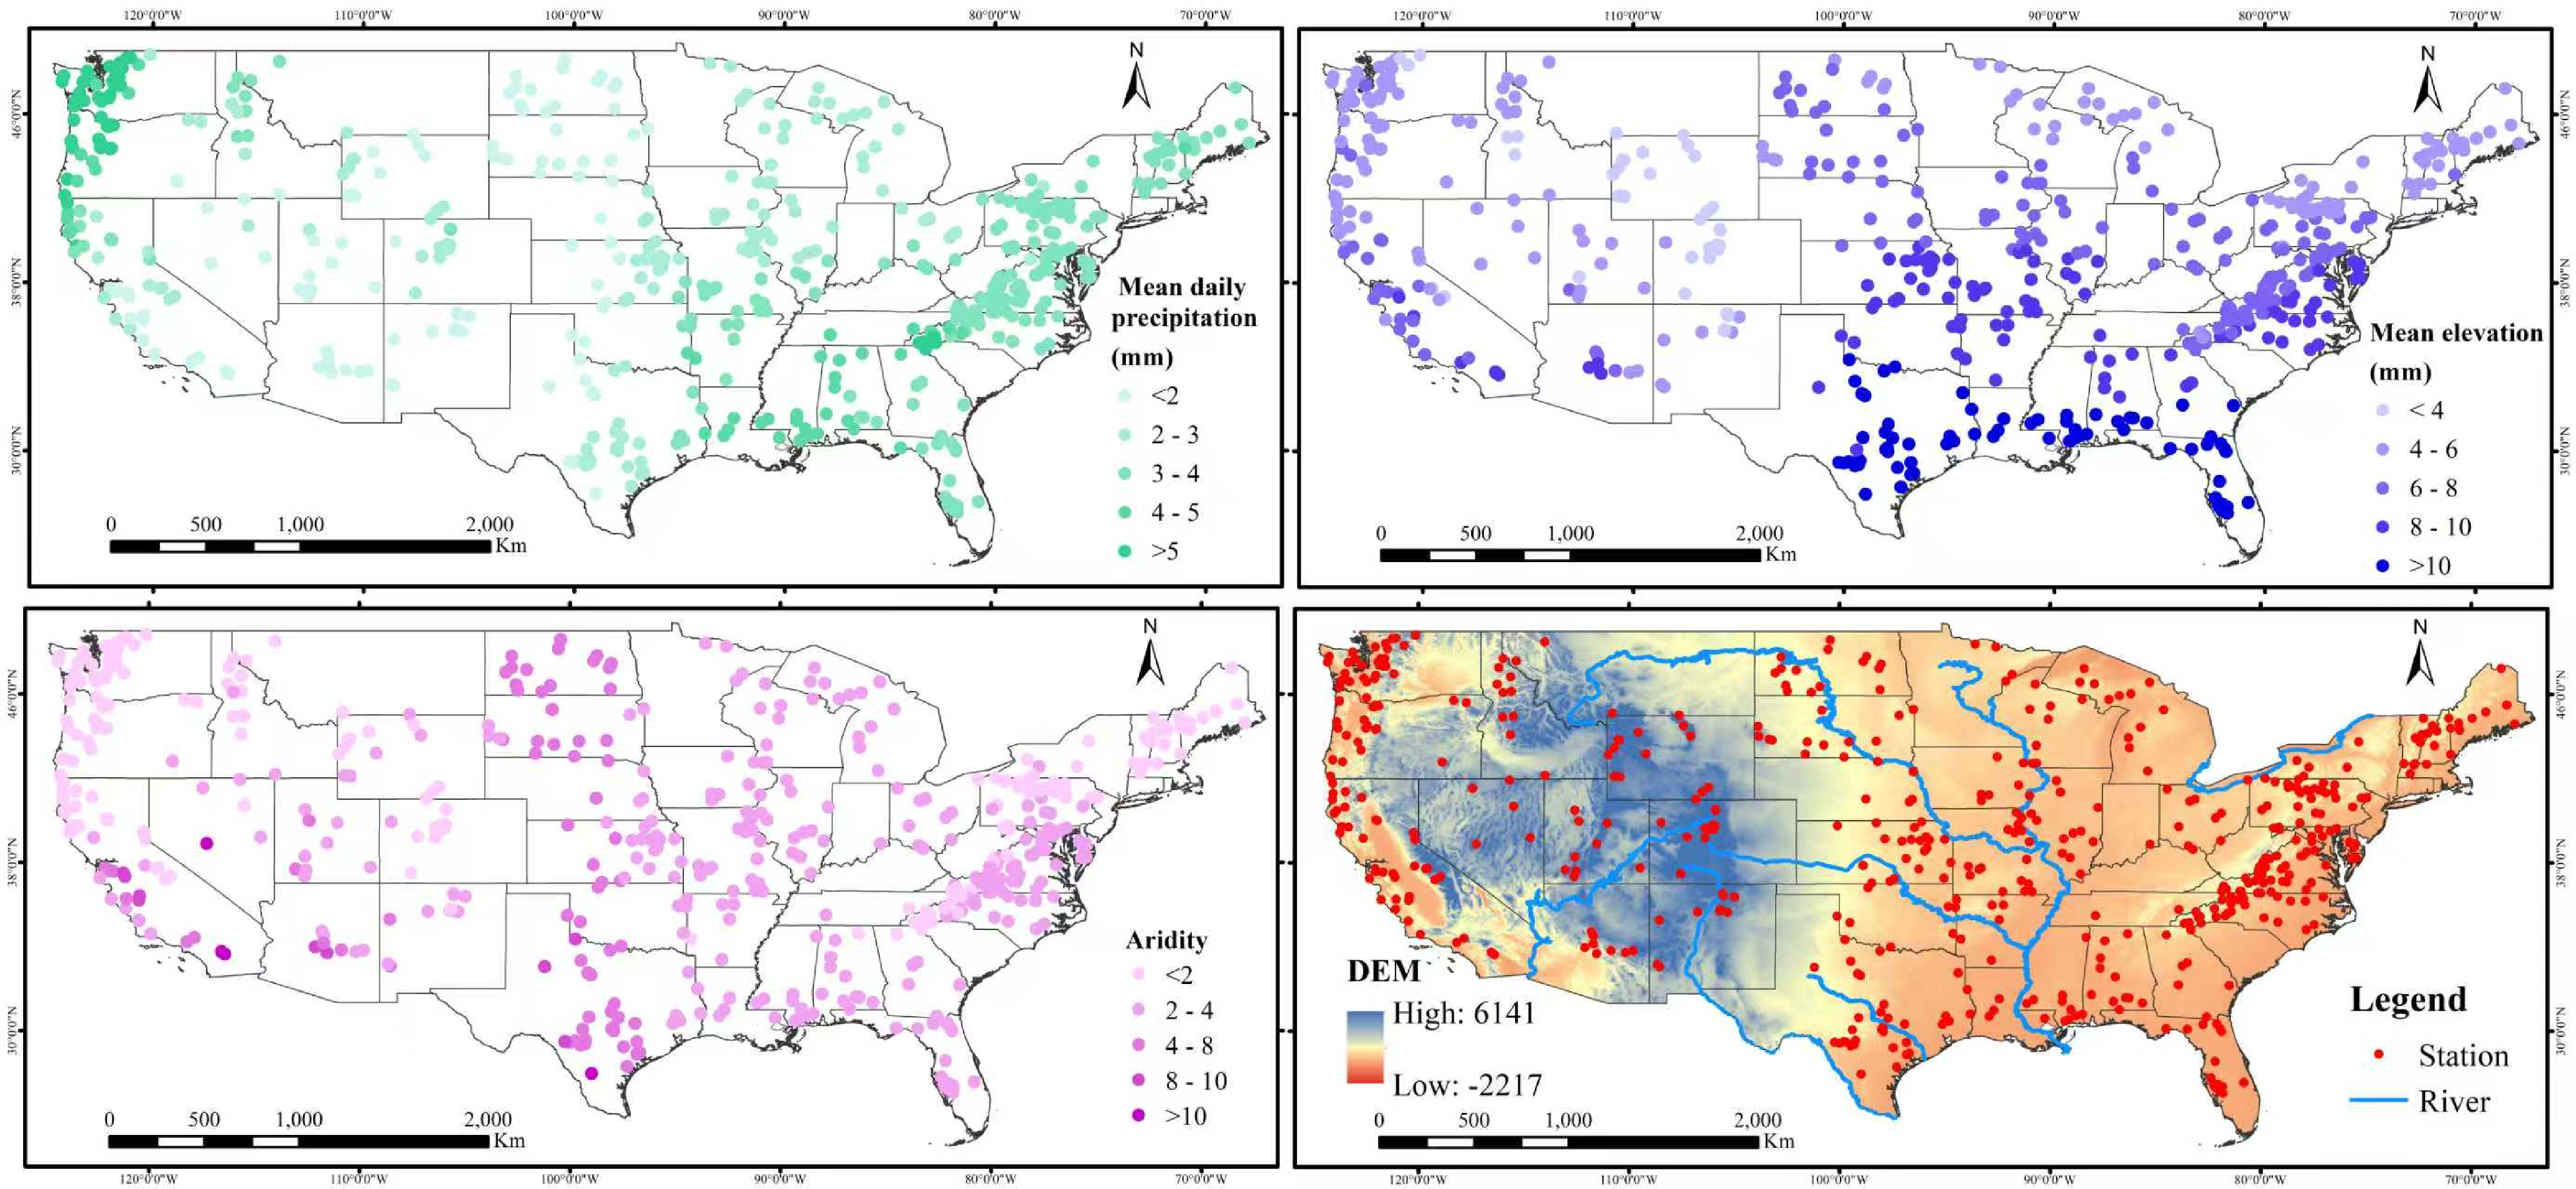
\includegraphics[width=\textwidth]{Figures/FigS1.pdf}
    \caption{
	Spatial distribution of selected streamflow stations after quality control
    }
    \label{fig:station}
\end{figure*}

The model input variables are summarized in Table~\ref{tab:input_features}. For each station, seven daily meteorological forcing variables from Daymet are used, and daily streamflow is additionally incorporated to represent antecedent hydrological state knowledge.

\begin{table}[htbp]
	\centering
	\caption{Selected Input Meteorological and Hydrological Variables}
	\label{tab:input_features}
	\begin{tabular*}{\textwidth}{@{\extracolsep{\fill}}lll}
		\toprule
		Group & Feature name & Unit \\
		\midrule
		\multirow{2}{*}{Energy} & day length (dayl) & s day$^{-1}$ \\
		& shortwave radiation (srad) & W m$^{-2}$ \\
		\multirow{2}{*}{Temperature} & maximum air temperature (tmax) & $^\circ$C \\
		& minimum air temperature (tmin) & $^\circ$C \\
		Atmospheric moisture & water vapour pressure (vp) & Pa \\
		Precipitation & precipitation (prcp) & mm day$^{-1}$ \\
		Snow & snow water equivalent (swe) & mm \\
		Runoff & streamflow (Q) & mm day$^{-1}$ \\
		\bottomrule
	\end{tabular*}
\end{table}

\section{Experimental Design and Detailed Settings}


\subsection{Parsimony and Physical Interpretability Are Prevalent}
\label{sec:parsimony}
\begin{table}[htbp]
    \centering
    \caption{Probe performance under different NSE conditions (without 1.5 IQR exclusion)}
    \begin{tabular*}{\textwidth}{@{\extracolsep{\fill}}llccc}
        \toprule
        Probe & Group & Mean & Median & p-value \\
        \midrule

        \multirow{3}{*}{$R^2_{\mathrm{cum}}$}
        & NSE $<$ 0.5    & -179546.7925 & 0.9610 & \multirow{3}{*}{0.8254} \\
        & NSE $\geq$ 0.5 & -1157736.4365 & 0.9537 & \\
        & All            & -793496.9145 & 0.9580 & \\

        \midrule

        \multirow{3}{*}{$R^2_{\mathrm{api}}$}
        & NSE $<$ 0.5    & -220124.9137 & 0.9659 & \multirow{3}{*}{0.6785} \\
        & NSE $\geq$ 0.5 & -1488511.0353 & 0.9601 & \\
        & All            & -1016213.7079 & 0.9632 & \\

        \midrule

        \multirow{3}{*}{$R^2_{\mathrm{chg}}$}
        & NSE $<$ 0.5    & -1064629.1571 & 0.4109 & \multirow{3}{*}{0.2355} \\
        & NSE $\geq$ 0.5 & -7409912.5486 & 0.4292 & \\
        & All            & -5047177.4662 & 0.4249 & \\

        \bottomrule
    \end{tabular*}

    \vspace{3pt}
    \begin{minipage}{\textwidth}
        \footnotesize
        \textit{Note:} No outlier exclusion was applied (full 521 stations). The strongly negative means are driven by a small number of extreme outliers in station-level $R^2$, whereas medians remain stable and representative of central tendency. p-values are computed by two-sided Mann--Whitney U tests between NSE groups.
    \end{minipage}
    \label{tab:probe_no_iqr_si}
\end{table}

\subsection{Learned Core Circuit Structures Reflect Hydrological Knowledge Across Basins}
\label{sec:knowledge}

To analyze how learned interaction structures in core circuits vary under different hydro-climatic conditions, we constructed multiple climate classification indicators based on static basin attributes, including aridity class, snow regime, and geo-climatic type\cite{hess-camels}. These classifications were used for post-hoc grouping and statistical analysis of interaction structures across basins.

\subsubsection*{Aridity Class}

Dryness conditions were classified using the aridity index (\texttt{aridity}) through binning\cite{zomer2022version}. The classification criteria are summarized in Table~\ref{tab:aridity_class}.

\begin{table}[htbp]
    \centering
    \caption{Aridity-based hydro-climatic classification}
    \label{tab:aridity_class}
    \begin{tabular*}{\textwidth}{@{\extracolsep{\fill}}lll}
        \toprule
        \textbf{Aridity range} & \textbf{Class} & \textbf{Description} \\
        \midrule
        $-1 \le aridity < 0.65$ & Arid & Arid \\
        $0.65 \le aridity < 1.0$ & Sub-humid & Sub-humid \\
        $aridity \ge 1.0$ & Humid & Humid \\
        \bottomrule
    \end{tabular*}
\end{table}

The thresholds (0.65 and 1.0) follow established hydro-climatic stratification practice and effectively distinguish energy-limited from water-limited basins\cite{hess-24-1081-2020}. They provide physically meaningful groupings for subsequent analysis of interaction structure distributions.

\subsubsection*{Snow Regime}

Snow regime was classified based on snowfall fraction (\texttt{frac\_snow}) to distinguish rain-dominated, mixed, and snow-influenced basins, as summarized in Table~\ref{tab:snow_regime}\cite{Berghuijs2014}.

\begin{table}[htbp]
    \centering
    \caption{Snow regime classification based on snowfall fraction}
    \label{tab:snow_regime}
    \begin{tabular*}{\textwidth}{@{\extracolsep{\fill}}lll}
        \toprule
        \textbf{Fraction range} & \textbf{Class} & \textbf{Description} \\
        \midrule
        $-0.1 \le frac\_snow < 0.1$ & Rain-dominant & Rain-dominated \\
        $0.1 \le frac\_snow < 0.3$ & Mixed & Mixed \\
        $frac\_snow \ge 0.3$ & Snow-influenced & Snow-influenced \\
        \bottomrule
    \end{tabular*}
\end{table}

The selected thresholds (0.1 and 0.3) reflect the gradual transition from rain-driven to snow-driven runoff. Low snowfall fractions correspond to basins dominated by direct rainfall, whereas higher fractions indicate increasing importance of snow accumulation and melt processes\cite{Biemans2019}.

\subsubsection*{Geo-climatic Type}

Geo-climatic type was determined using a hierarchical rule based on elevation (\texttt{forcing\_elev\_m}), longitude (\texttt{lon}), and aridity\cite{hess-24-1081-2020}. The pseudocode is shown in Algorithm~\ref{alg:geo_climate}.

\begin{algorithm}[htbp]
    \caption{Hierarchical classification for geo-climatic type}
    \label{alg:geo_climate}
    \begin{algorithmic}[1]
        \Require Elevation $forcing\_elev\_m$, Longitude $lon$, Aridity $aridity$
        \Ensure Geo-climatic type $geo\_climate\_type$
        \If{$forcing\_elev\_m \ge 1500$}
        \State $geo\_climate\_type \gets \text{"Plateau/Mountain"}$
        \ElsIf{$lon \le -120$}
        \State $geo\_climate\_type \gets \text{"Oceanic"}$
        \ElsIf{$aridity \ge 1.5$}
        \State $geo\_climate\_type \gets \text{"Arid Continental"}$
        \Else
        \State $geo\_climate\_type \gets \text{"Humid Continental/Subtropical"}$
        \EndIf
    \end{algorithmic}
\end{algorithm}

This hierarchical classification first identifies high-elevation regions ($\geq 1500 m$), then distinguishes oceanic versus inland climates based on longitude, and finally separates arid continental basins using a higher aridity threshold (1.5). This approach provides a physically interpretable stratification of basins across major hydro-climatic regimes.

\subsection{Accurate Volume Response but Limited Sensitivity to Temporal and State Perturbations}
\label{sec:sensitive}

To examine whether the model encodes physically consistent hydrological sensitivities—rather than relying on spurious statistical correlations—we designed a station-wise counterfactual sensitivity framework on the test split\cite{simic2025perturbation}. Let $f_{\theta}$ denote the trained sparse transformer, $\mathbf{X}_{i}\in\mathbb{R}^{N_i\times L\times F}$ the input tensor for station $i$ (with $N_i$ samples, lookback length $L$, and $F$ predictors), and $\mathbf{y}_{i}\in\mathbb{R}^{N_i}$ the observed discharge target. For each intervention setting $s$, we define
\begin{equation}
    \hat{\mathbf{y}}_{i}^{(0)} = f_{\theta}(\mathbf{X}_{i}),
    \qquad
    \hat{\mathbf{y}}_{i}^{(s)} = f_{\theta}(\mathcal{T}_{s}(\mathbf{X}_{i})),
\end{equation}
where $\mathcal{T}_{s}(\cdot)$ denotes an intervention operator applied in physical space and subsequently mapped back to the normalized model space using the same normalization statistics as in training\cite{read2019process}. This paired design isolates the model’s response to controlled perturbations while eliminating cross-sample confounding effects\cite{10.2166/wcc.2017.149}.

\subsubsection*{Experiment design}

We considered four intervention families to disentangle model sensitivities to hydrological drivers, including volume, temporal distribution, catchment state, and thermal forcing\cite{hess-30-1077-2026}. The perturbation ranges are chosen to represent moderate yet plausible deviations that remain within the support of the training distribution.

\paragraph{(1) Rainfall scaling.}
Let $P_t$ denote precipitation at lag $t\in\{1,\dots,L\}$. With scaling factor $\alpha$, the intervention is
\begin{equation}
    P_t' = \alpha P_t,
    \qquad
    \alpha\in\{0.8,0.9,1.1,1.2\}.
\end{equation}
This modifies storm magnitude while preserving the original temporal structure of rainfall\cite{nearing2021role}.

\paragraph{(2) Rainfall pattern redistribution.}
Let $\mathbf{w}^{(m)}=(w_1^{(m)},\dots,w_L^{(m)})$ be a mode-specific nonnegative weight vector (front-loaded, middle-loaded, back-loaded, uniform) satisfying $\sum_{t=1}^{L}w_t^{(m)}=1$. The redistributed rainfall is
\begin{equation}
    P_t' = \Big(\sum_{j=1}^{L}P_j\Big) w_t^{(m)}.
\end{equation}
This conserves total rainfall volume while altering its temporal distribution within the input window\cite{Wrr_p_q}. We note that this intervention represents an idealized redistribution rather than a physically simulated storm evolution, and is intended to isolate model sensitivity to intra-window timing patterns.

\paragraph{(3) Streamflow-input scaling (state perturbation).}
Let $Q_t^{\mathrm{in}}$ denote the lagged streamflow input channel. With scaling factor $\beta$,
\begin{equation}
    Q_t^{\mathrm{in}\prime} = \beta Q_t^{\mathrm{in}},
    \qquad t=1,\dots,L,
    \qquad
    \beta\in\{0.1,0.5,0.9,1.1,1.5,1.9\}.
\end{equation}
This isolates sensitivity to hydrological state magnitude in the full lookback window while preserving the original temporal pattern\cite{apak2026multi}.

\paragraph{(4) Temperature increase perturbation.}
For each temperature-related predictor $T_t$, we apply
\begin{equation}
    T_t' = T_t + \Delta T,
    \qquad
    \Delta T\in\{3,5,7\}^{\circ}\mathrm{C}.
\end{equation}
This probes thermal forcing effects (e.g., evapotranspiration or snowmelt processes), particularly in energy-limited or snow-influenced catchments\cite{milly2020colorado}.

In total, the intervention set contains $4+4+6+3=17$ scenarios per station. For each station and scenario, responses are computed against the same baseline prediction, enabling paired comparison\cite{LouiseSlater2024_XAI_Hydrology}.

\subsubsection*{Evaluation metrics}

For station $i$ and scenario $s$, with sample-wise observations $y_{i,n}$ and predictions $\hat y_{i,n}^{(s)}$ ($n=1,\dots,N_i$), we evaluate the following metrics\cite{WRR_RMSE,Nse}: \textbf{(1) MSE.}

\paragraph{(2) Predicted streamflow volume.}
\begin{equation}
    V_{i}^{(s)} = \sum_{n=1}^{N_i}\hat y_{i,n}^{(s)}.
\end{equation}

\paragraph{(3) Predicted peak timing index.}
\begin{equation}
    \tau_{i}^{(s)} = \arg\max_{1\le n\le N_i}\hat y_{i,n}^{(s)}.
\end{equation}
Peak-timing-based diagnostics are commonly used to characterize flow timing shifts under altered hydro-climatic forcing\cite{bloschl2017changing}.

Relative to baseline $s=0$, we define
\begin{equation}
    \Delta\mathrm{MSE}_{i}^{(s)} = \mathrm{MSE}_{i}^{(s)}-\mathrm{MSE}_{i}^{(0)},
    \quad
    \Delta V_{i}^{(s)} = V_{i}^{(s)}-V_{i}^{(0)},
    \quad
    \Delta\tau_{i}^{(s)} = \tau_{i}^{(s)}-\tau_{i}^{(0)}.
\end{equation}

For visualization comparability across stations, relative changes are reported as
\begin{equation}
    \delta\mathrm{MSE}_{i}^{(s)}(\%) = 100\times\frac{\Delta\mathrm{MSE}_{i}^{(s)}}{\max\big(|\mathrm{MSE}_{i}^{(0)}|,1\big)},
    \qquad
    \delta V_{i}^{(s)}(\%) = 100\times\frac{\Delta V_{i}^{(s)}}{\max\big(|V_{i}^{(0)}|,1\big)}.
\end{equation}

\subsubsection*{Physical consistency criteria}

To assess whether model responses align with expected hydrological behavior, we adopt direction-based consistency criteria\cite{read2019process}:

For rainfall scaling and streamflow-input scaling, expected behavior requires directionally consistent changes in streamflow volume, i.e., $\Delta V$ increases for scaling factors greater than 1 and decreases for factors less than 1\cite{nearing2021role}.

For rainfall pattern redistribution and temperature perturbation, expected behavior requires that model performance does not exhibit systematic degradation, i.e., no consistent increase in prediction error across scenarios\cite{hess-30-1077-2026}.

Finally, for each intervention family, station-level expectedness is aggregated by majority vote over its scenarios. Statistical significance of paired scenario effects is assessed by two-sided Wilcoxon signed-rank tests, with Benjamini--Hochberg correction for multiple comparisons.

\subsection{STEH-Derived Interpretability Enhances Random Forest Predictive Performance}
\label{sec:rfDesign}
To evaluate whether the hydrological circuit structures revealed by STEH can improve a conventional machine-learning benchmark, we designed a paired station-wise comparison between a \emph{baseline} Random Forest (RF) and a \emph{STEH-informed modified} RF\cite{hess-25-2997-2021}. Both models are trained and tested on the same station, temporal split, and target variable, ensuring that any performance differences can be attributed to the STEH-derived design rather than inconsistencies in data or experimental setup\cite{ABBASI2021125717}.

Let station index be $i\in\{1,\dots,M\}$, predictors $\mathbf{X}_i$, and discharge target $\mathbf{y}_i$. For each station, we train
\begin{equation}
    \hat{\mathbf{y}}^{\text{base}}_i = g_{\phi_i}(\mathbf{X}_i),
    \qquad
    \hat{\mathbf{y}}^{\text{mod}}_i = g_{\psi_i}(\widetilde{\mathbf{X}}_i),
\end{equation}
where $g_{\phi_i}$ and $g_{\psi_i}$ denote RF predictors with station-specific fitted parameters.

\subsubsection*{Experiment design}

During model training, the hyperparameters of both Random Forest models are optimized using Bayesian optimisation on the validation set\cite{BO_OPT}, ensuring that performance differences are not attributable to discrepancies in tuning strategy. Specifically, the tuned hyperparameters include tree depth ($\in [2, 8]$), the minimum number of samples required for node splitting ($\in [2, 8]$), the minimum number of samples at leaf nodes ($\in [1, 4]$), and the feature sampling ratio for split selection ($\in [0.5, 0.8]$). Further details are provided in Supplementary Notes \ref{sec:rfHyper}.

The task is formulated as a one-step-ahead prediction problem, where a fixed 10-day input window is used to predict next-day discharge. Both baseline and modified models use the same input length ($L=10$). Data are split chronologically into training, validation, and testing sets with ratios of $0.7/0.15/0.15$, respectively, on a per-station basis. Both models use identical raw drivers, including precipitation, temperature, shortwave radiation, and antecedent discharge.

\paragraph{Baseline RF.}
The baseline model adopts standard lagged inputs and rolling statistical summaries, without incorporating explicit hydrological regime information.

\paragraph{STEH-informed modified RF.}
The modified model incorporates structural insights revealed by STEH (primarily P--Q, Q--Q, and T--Q pathways). Specifically, it includes physically interpretable aggregated features (e.g., $P_{3}, P_{7}, P_{14}, Q_{3}, Q_{7}, Q_{3}-Q_{7}, T_{7}^{+}, T_{7}^{-}$), introduces regime indicators to distinguish dominant hydrological processes (P--Q, Q--Q, T--Q), and applies light regime-aware sample weighting for selected regimes (P--Q and T--Q) during training.

The dominant regime for each station is identified over the training period based on correlation analysis\cite{Wrr_p_q}. Specifically, we compute
\begin{equation}
    r_{\mathrm{PQ}} = \mathrm{corr}(P_t, Q_t),
    \quad
    r_{\mathrm{QQ}} = \mathrm{corr}(Q_{t-1}, Q_t),
    \quad
    r_{\mathrm{TQ}} = \mathrm{corr}(T_t, Q_t),
\end{equation}
and define the regime as
\begin{equation}
    \mathcal{R}_i = \arg\max\{r_{\mathrm{PQ}}, r_{\mathrm{QQ}}, r_{\mathrm{TQ}}\}.
\end{equation}
This regime label is then used as part of the model input.

\subsubsection*{Training and evaluation protocol}

Model performance is evaluated using Nash--Sutcliffe efficiency (NSE), mean squared error (MSE), and mean absolute error (MAE), with test NSE serving as the primary comparison metric\cite{Nse}. Evaluation is conducted on stations where the sparse-transformer benchmark achieves NSE greater than 0.5\cite{WRR_NSE}.

For the selected stations, we report the mean NSE, mean MSE and mean MAE of both baseline and modified RF models, and perform paired t-test and Wilcoxon signed-rank test on station-wise NSE differences.

\section{Model Hyperparameters}
\subsection{STEH}
\label{sec:STEHhyper}

Hyperparameters were systematically optimized within the predefined search spaces listed in Table \ref{tab:hyperparameters}\cite{BO_OPT}, ensuring reproducibility and minimizing subjective bias. The sparsity-related settings are consistent with prior sparse-Transformer practice\cite{openai_weight_sparse_transformers}.

Due to the large number of study sites, reporting all optimized hyperparameter configurations in this Supplementary Information is impractical. Therefore, the complete set of best hyperparameters is provided in an repository for full transparency and reproducibility:\href{https://github.com/Polyethylenekjc/Sparse-Transformer-In-Streamflow-Prediction/blob/main/outcomes/STEH\_Best\_Hyperparams.csv}{https://github.com/Polyethylenekjc/Sparse-Transformer-In-Streamflow-Prediction/blob/main/outcomes/STEH\_Best\_Hyperparams.csv}


\begin{table}[htbp]
    \centering
    \caption{Hyperparameter settings and search space}
    \label{tab:hyperparameters}
    \begin{tabular*}{\textwidth}{@{\extracolsep{\fill}}lll}
        \toprule
        \textbf{Hyperparameter} & \textbf{Description} & \textbf{Search Space} \\
        \midrule
        Learning rate & Controls optimisation step size & $10^{-4}$ -- $10^{-2}$ \\
        Batch size & Number of samples per mini-batch & $32$ -- $256$ \\
        Hidden size & Dimension of hidden representations & $16$ -- $256$ \\
        Number of layers & Number of Transformer encoder layers & $1$ -- $16$ \\
        Weight sparsity & Target fraction of pruned weights in Stage II & $0.7$ -- $0.95$ \\
        Activation sparsity & Sparsification applied on the last activation dimension. & $0.6$ -- $0.9$ \\
        Gate regularisation & Strength of gate sparsity regularization & $10^{-5}$ -- $10^{-3}$ \\
        \bottomrule
    \end{tabular*}
\end{table}

\subsection{Random Forest}
\label{sec:rfHyper}
Hyperparameters of the Random Forest models were systematically optimized using Bayesian optimisation within the predefined search spaces listed in Table \ref{tab:rf_hyperparameters}\cite{BO_OPT}, ensuring reproducibility and minimizing subjective bias.

Due to the large number of study sites, reporting all optimized hyperparameter configurations in this Supplementary Information is impractical. Therefore, the complete set of best hyperparameters is provided in a repository for full transparency and reproducibility: \href{https://github.com/Polyethylenekjc/Sparse-Transformer-In-Streamflow-Prediction/blob/main/outcomes/Rf\_Best\_Hyperparams.csv}{https://github.com/Polyethylenekjc/Sparse-Transformer-In-Streamflow-Prediction/blob/main/outcomes/Rf\_Best\_Hyperparams.csv}

\begin{table}[htbp]
    \centering
    \caption{Hyperparameter settings and search space for Random Forest}
    \label{tab:rf_hyperparameters}
    \begin{tabular*}{\textwidth}{@{\extracolsep{\fill}}lll}
        \toprule
        \textbf{Hyperparameter} & \textbf{Description} & \textbf{Search Space} \\
        \midrule
        Tree depth & Maximum tree depth & $2$ -- $8$ \\
        Min samples (split) & Minimum number of samples required to split & $2$ -- $8$ \\
        Min samples (leaf) & Minimum number of samples per leaf & $1$ -- $4$ \\
        Feature ratio & Fraction of features considered per split & $0.5$ -- $0.8$ \\
        \bottomrule
    \end{tabular*}

    \vspace{2mm}
    \footnotesize
    \textit{Note:} ``Baseline'' refers to the standard Random Forest model without incorporating STEH-derived hydrological knowledge, while ``Modified'' denotes the Random Forest model augmented with STEH-informed structured features.
\end{table}

\bibliographystyle{unsrtnat}
\bibliography{reference}

\end{document}
